\documentclass[nofootinbib,twocolumn,showpacs,prl,superscriptaddress,secnumarabic,amssymb,nobibnotes,aps,floatfix]{revtex4}
\usepackage{graphicx}
\usepackage{hyperref}
%
\def\Dirac#1{#1\hskip-5pt/}
%
\begin{document}

\title{First Exclusive Measurement of Deep Virtual Compton Scattering off $^4$He: Toward the 3D tomography of nuclei}

\newcommand*{\ANL}{Argonne National Laboratory, Argonne, Illinois 60439}
\newcommand*{\ANLindex}{1}
\affiliation{\ANL}
\newcommand*{\ORSAY}{Institut de Physique Nucl\'eaire, CNRS/IN2P3 and Universit\'e Paris Sud, Orsay, France}
\newcommand*{\ORSAYindex}{2}
\affiliation{\ORSAY}
\newcommand*{\JLAB}{Thomas Jefferson National Accelerator Facility, Newport News, Virginia 23606}
\newcommand*{\JLABindex}{3}
\affiliation{\JLAB}
 
\newcommand*{\NOWJLAB}{Thomas Jefferson National Accelerator Facility, Newport News, Virginia 23606}
\newcommand*{\NOWODU}{Old Dominion University, Norfolk, Virginia 23529}
 %%%%%%%%%%%%%%% END OF Latex Macros for institute addresses  %%%%%%%%%%%%%%%%%%%%%%%%% 

\author {M.~Hattawy}
\affiliation{\ANL}
\affiliation{\ORSAY}
\author {R.~Dupr\'{e}} 
\affiliation{\ANL}
\affiliation{\ORSAY}
\author {N.A.~Baltzell} 
\affiliation{\ANL}
\affiliation{\JLAB}
\author {K.~Hafidi} 
\email[corresponding author: ]{kawtar@anl.gov}
\affiliation{\ANL}


\collaboration{The CLAS Collaboration}
\noaffiliation

%
\date{\today}
%
\begin{abstract}
We report the first exclusive measurements of deeply virtual Compton scattering (DVCS) off a nucleus, where all the products of the reaction including the recoil $^4$He nucleus were detected. The experiment was performed using the Jefferson Lab CEBAF Large Acceptance Spectrometer (CLAS) enhanced with a radial time projection chamber (RTPC) to detect the recoiling $^4$He nuclei. We measure large beam spin asymmetries comparable to the proton's ones and extract in a model independent way, the single chirally-even generalized parton distribution of the $^4$He nucleus. These are pioneering measurements and will lead the way toward the 3D imaging of the partonic structure of nuclei. 
\end{abstract}
\pacs{Valid PACS appear here}

\maketitle 

A wealth of information on the quantum chromodynamics (QCD) structure of hadrons lies in the correlations between the momentum and spatial degrees of freedom of the constituent partons. Such correlations are accessible via the generalized parton distributions (GPDs). The GPDs correspond to the coherence between quantum states of different (or same) helicity, longitudinal momentum, and transverse position. In an impact parameter space, they can be interpreted as a distribution in the transverse plane of partons carrying a certain longitudinal momentum \cite{Burkardt:2000za,Diehl:2002he,Belitsky:2002ep}. A crucial feature of GPDs is the access to the transverse position of partons which, combined with their longitudinal momentum, leads to the total angular momentum of partons \cite{Burkardt:2005hp}. Deep virtual Compton scattering (DVCS) corresponding to hard exclusive electroproduction of a real photon, is considered the cleanest probes to access GPDs and thus study the 3D imaging of nucleons and nuclei.

DVCS measurements have been the focus of a worldwide effort \cite{Stepanyan:2001sm,Airapetian,Chekanov:2003ya,Aktas:2005ty,Chen:2006na,Munoz Camacho:2006hx,Girod:2007aa,Gavalian:2009,Seder:2015,Pisano:2015,Jo:2015ema} involving several accelerator facilities such as Jefferson Lab (JLab), HERA and  CERN. The vast majority of the experiments focused on the study of the nucleon's structure. The deuterium was also investigated at HERMES and JLab \cite{Mazouz:2007aa} mainly as a neutron target. Studying the 3D imaging of the nucleon is terms of its fundamental constituents is a very important goal. Understanding how these distributions are modified to provide the binding and structure in a nucleus is as fascinating of a question and an integral part of our quest of using QCD to explore nuclear matter. The study of nuclear DVCS is still in its infancy due to the challenging detection of the low energy recoil nucleus. Until very recently, the HERMES experiment \cite{Ellinghaus:2002zw} was the only one to measure DVCS off heavier nuclei such as $^4$He, N, Ne, Kr and Xe, where only the scattered electron and the real photon are detected. In this paper, we report the first exclusive measurements of DVCS off $^4$He where all products of the reaction are detected including the recoiling $^4$He nucleus.



\begin{figure}[tb]
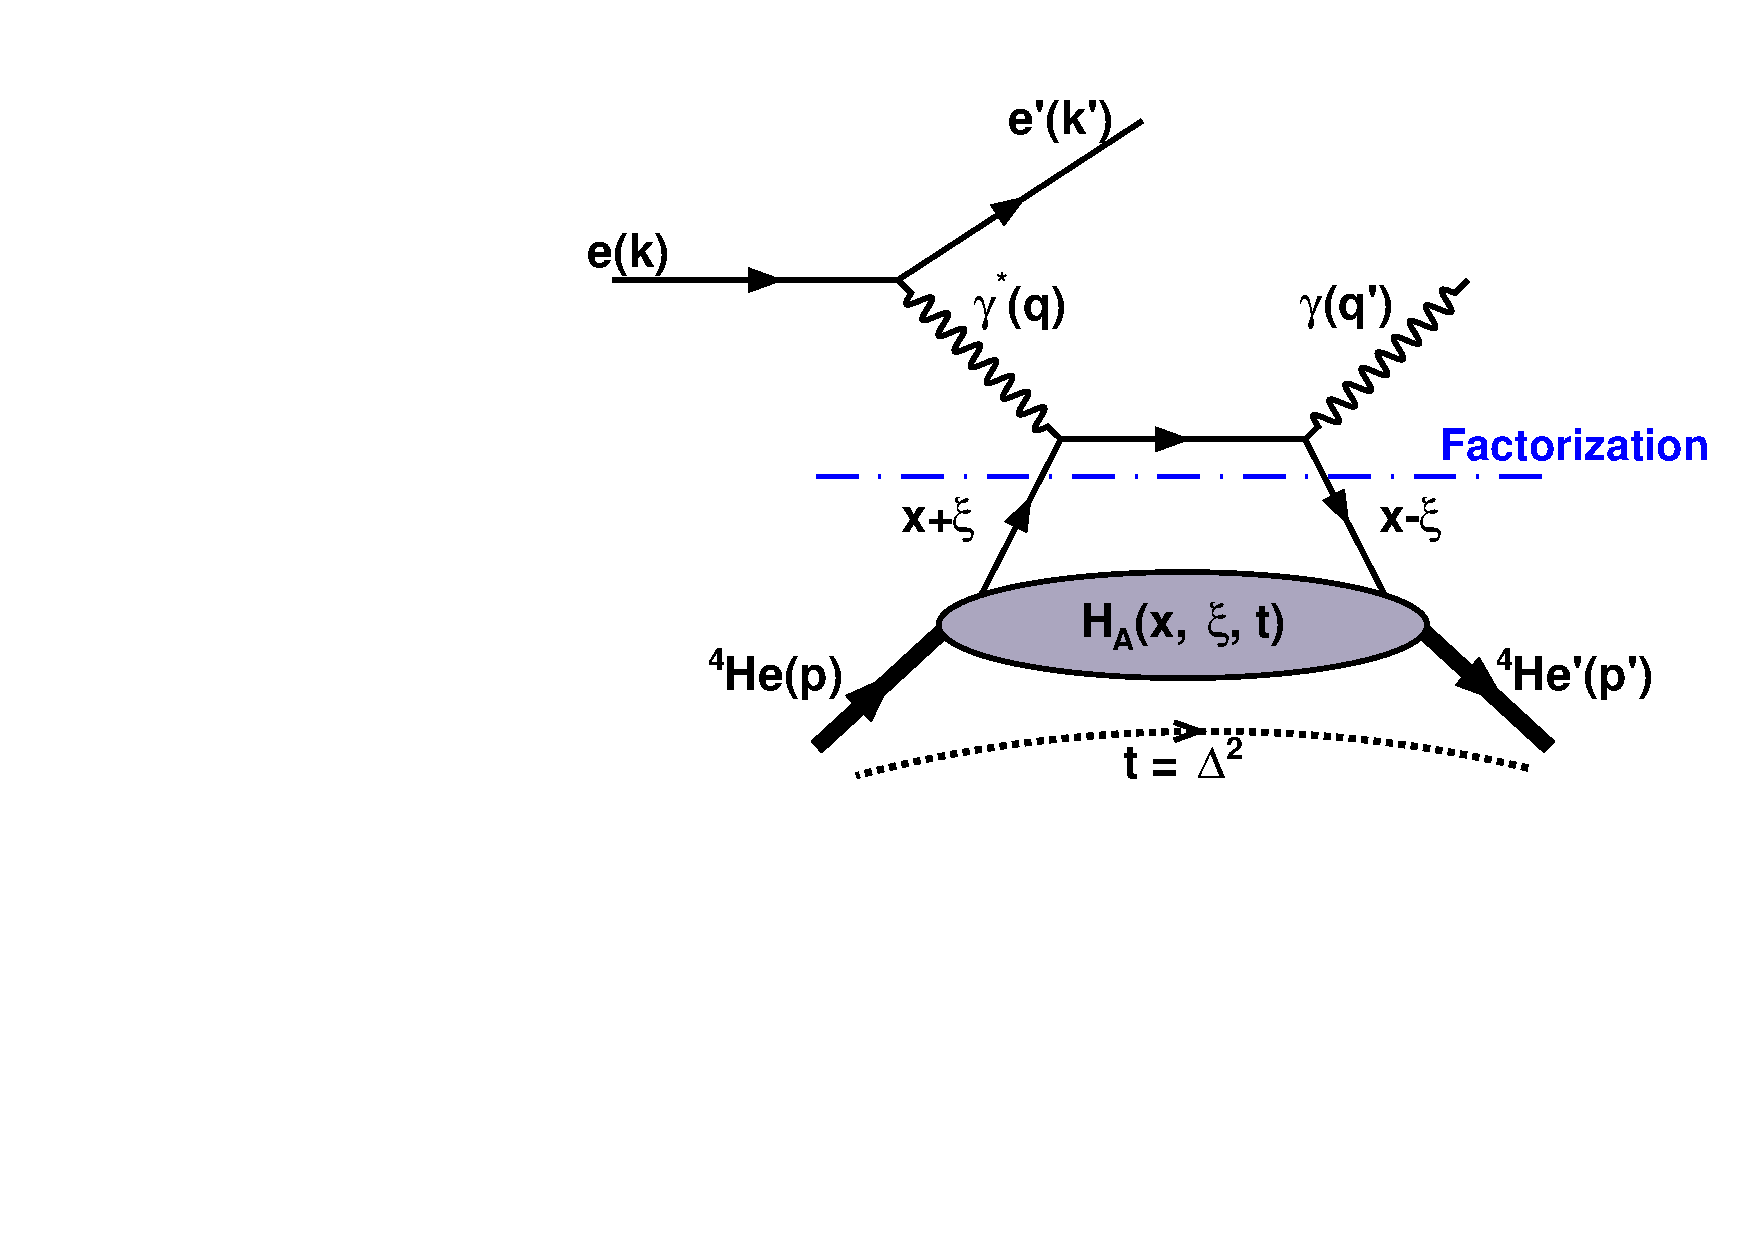
\includegraphics[width=6.5cm]{figs/DVCS_diagram.pdf}
\vspace{-0.cm}
\caption{Deep virtual Compton scattering process in the handbag approximation.}
\label{fig:diags}
\end{figure}

\begin{figure}[tb]
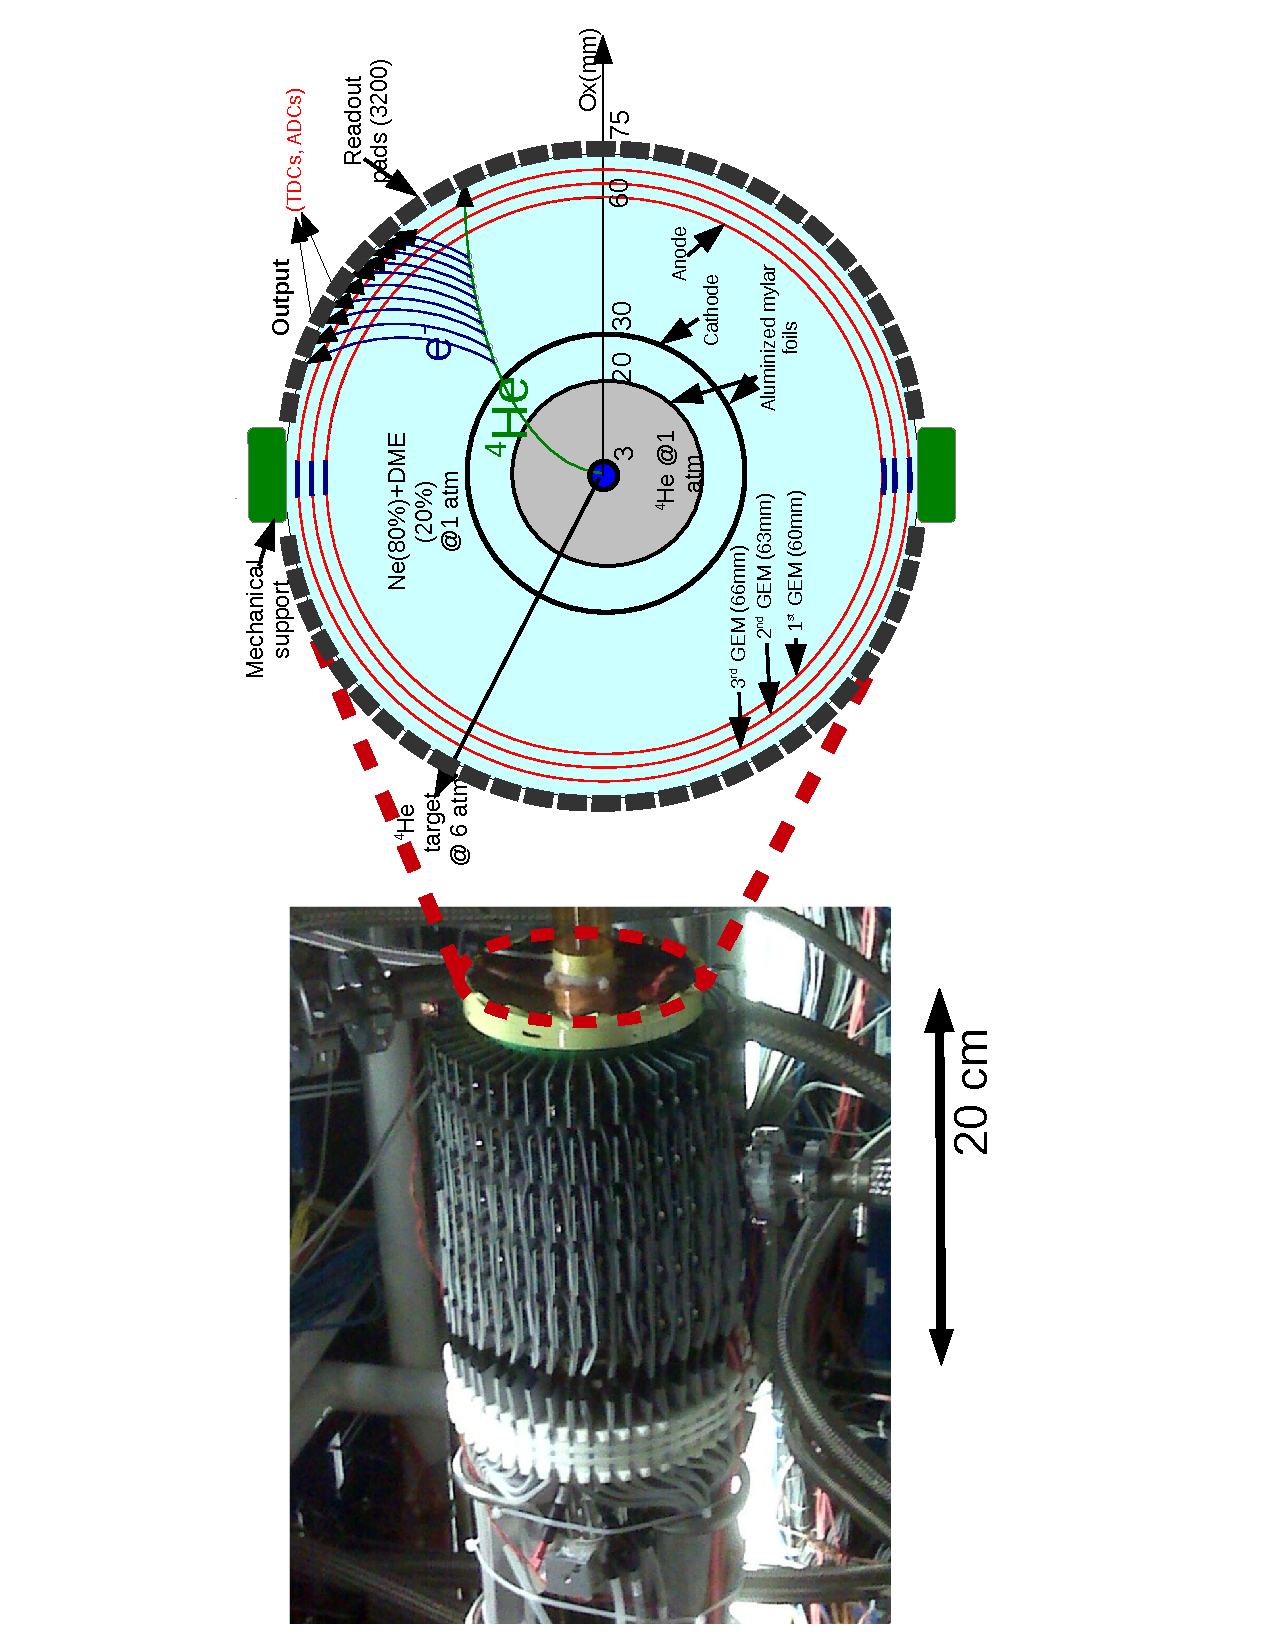
\includegraphics[width=6.5cm,angle=-90]{figs/RTPC.pdf}
\vspace{-0.9cm}
\caption{Left: A picture of the \it{eg6} RTPC before insertion into the solenoid. Right: A cross section of the \it{eg6} RTPC perpendicular to the beam direction. An illustration of a $^4$He track originating from the pressurized straw target is shown along with the electrons produced in the drift region.}
\label{fig:RTPC}
\end{figure}

\begin{figure}[tb]
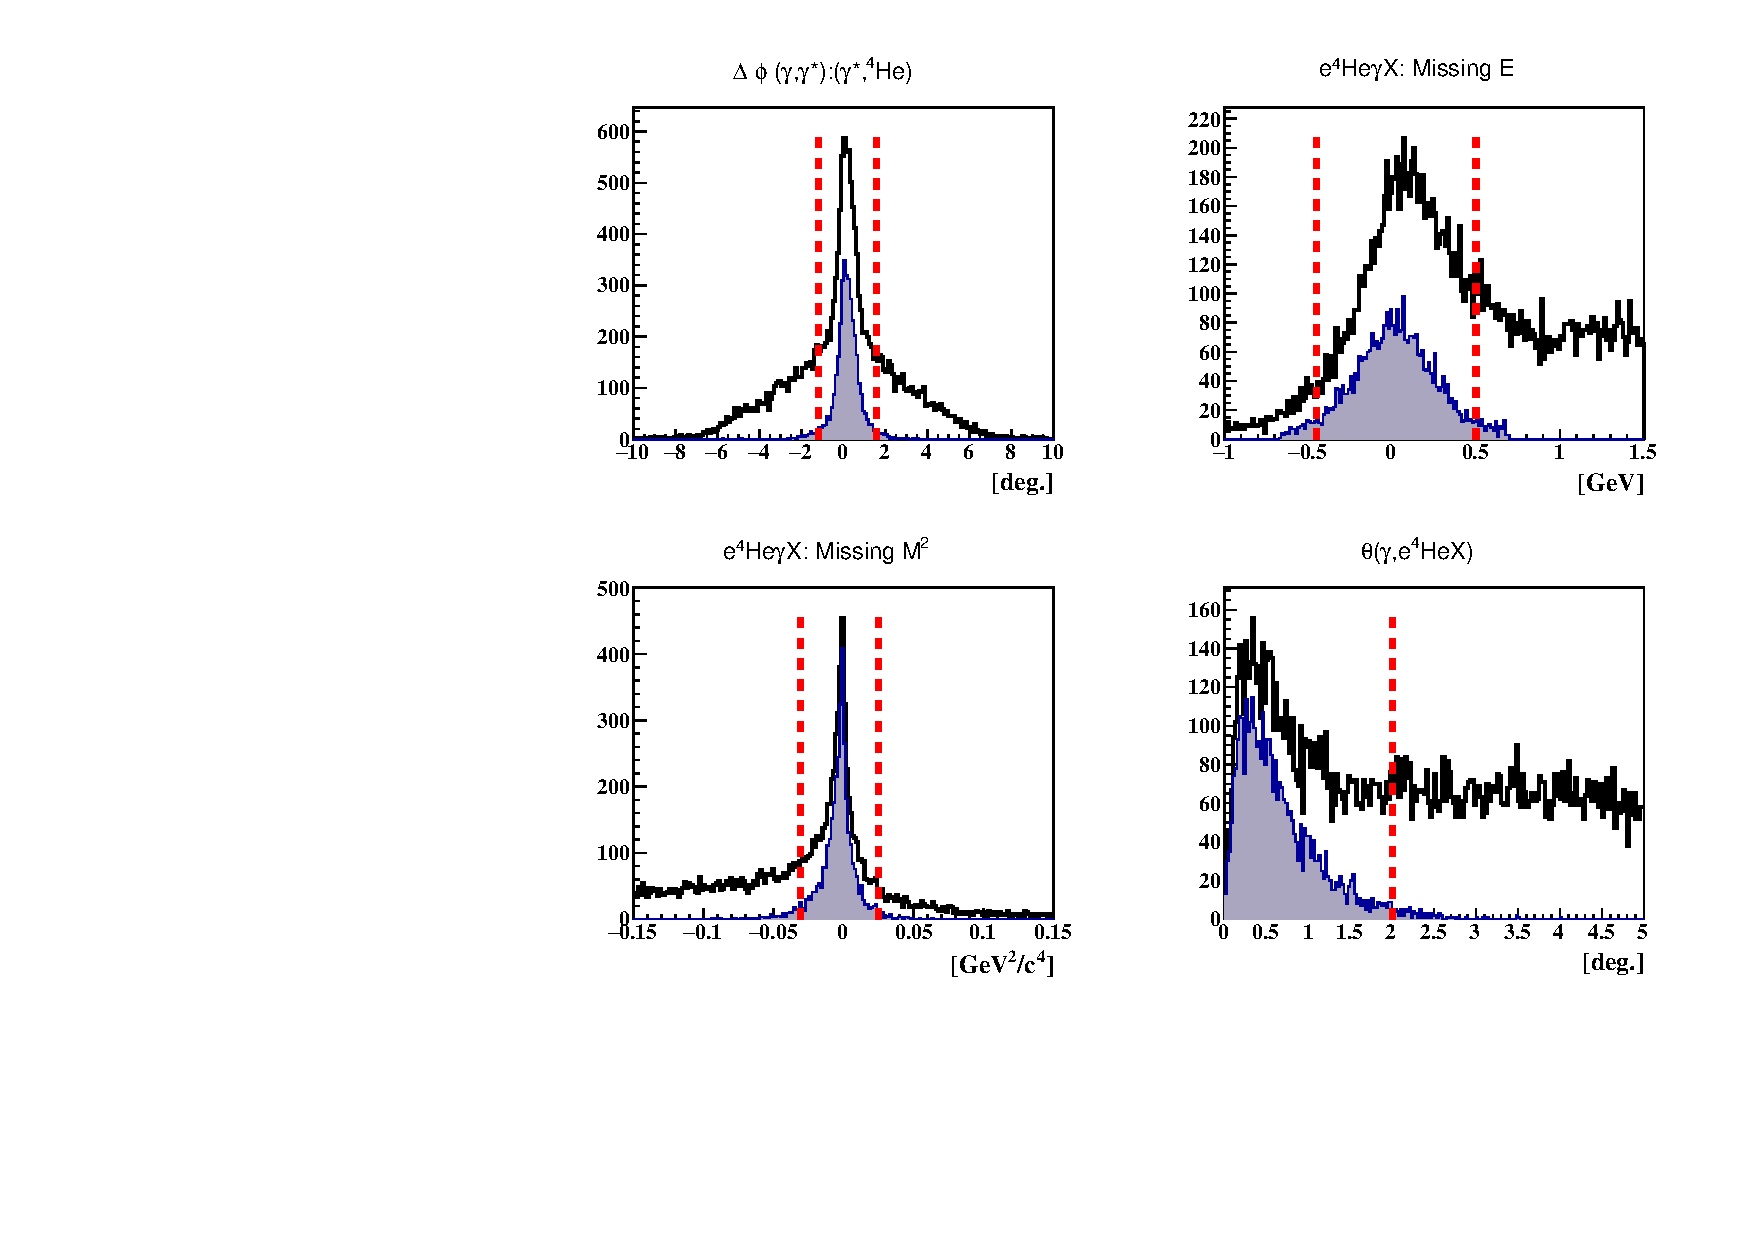
\includegraphics[width=8.9cm]{figs/coh_exc_cuts.pdf}
\vspace{-0.9cm}
\caption{}
\label{fig:kin-cuts}
\end{figure}


\begin{figure}[tb]
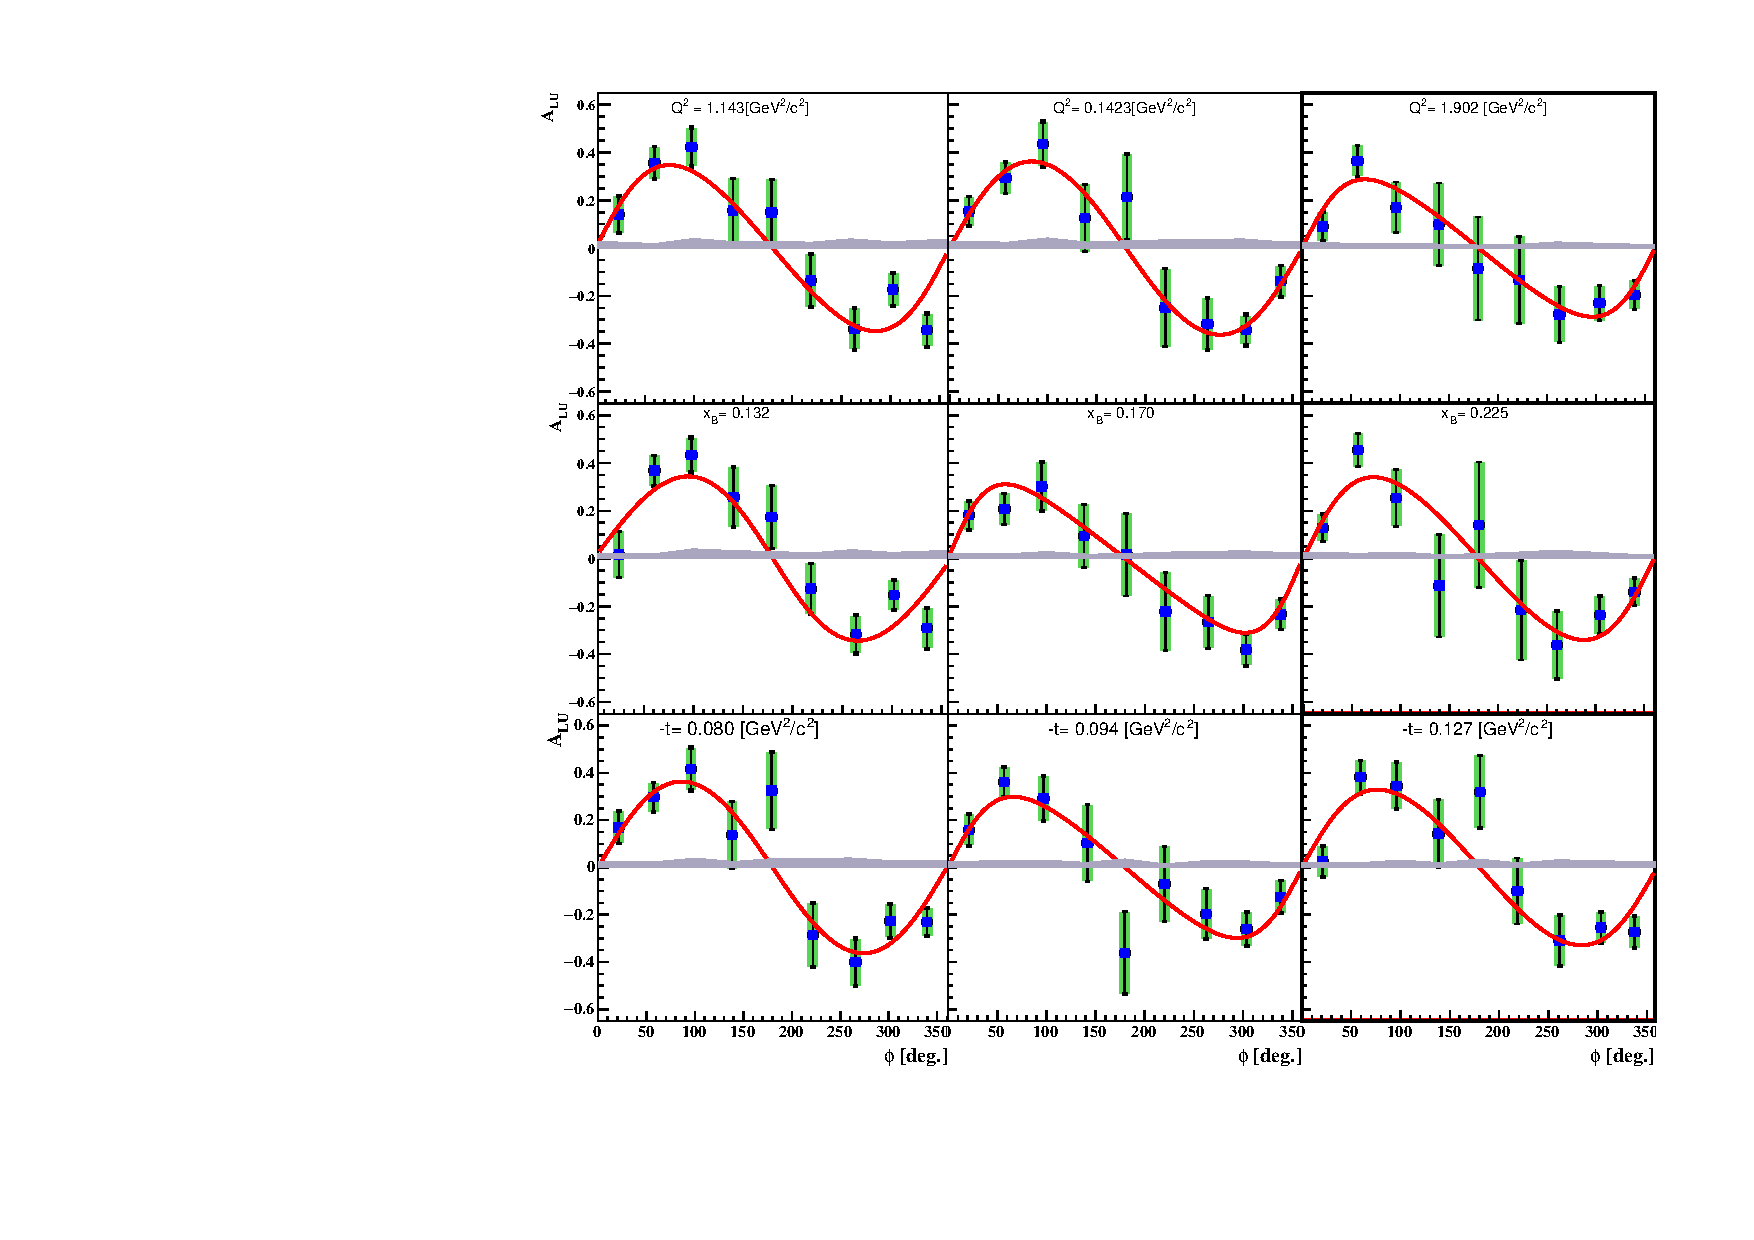
\includegraphics[width=8.9cm]{figs/coherent-ALU.pdf}
\vspace{-0.9cm}
\caption{}
\label{fig:alu}
\end{figure}

\begin{figure}[tb]
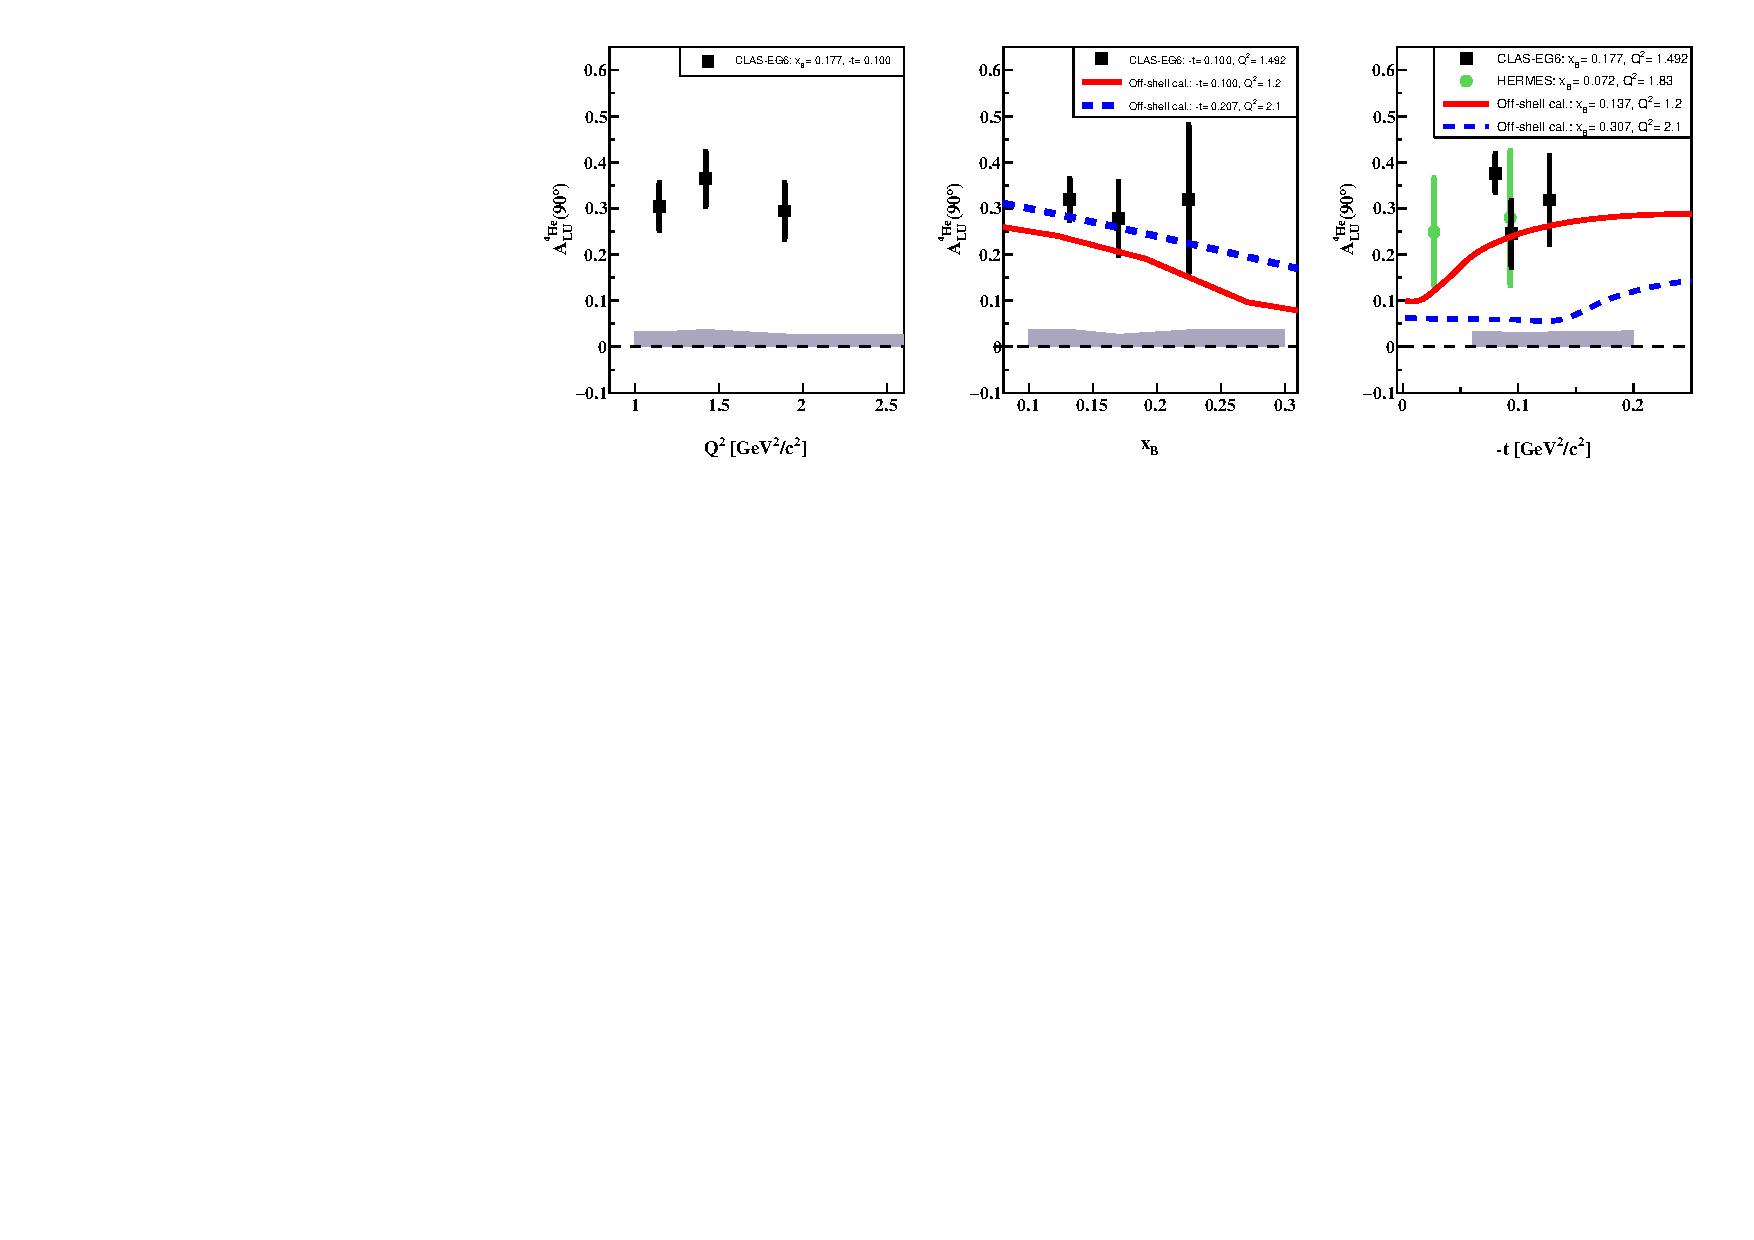
\includegraphics[width=8.9cm]{figs/coherent-ALU_90.pdf}
\vspace{-0.9cm}
\caption{}
\label{fig:alu90}
\end{figure}


\begin{figure}[tb]
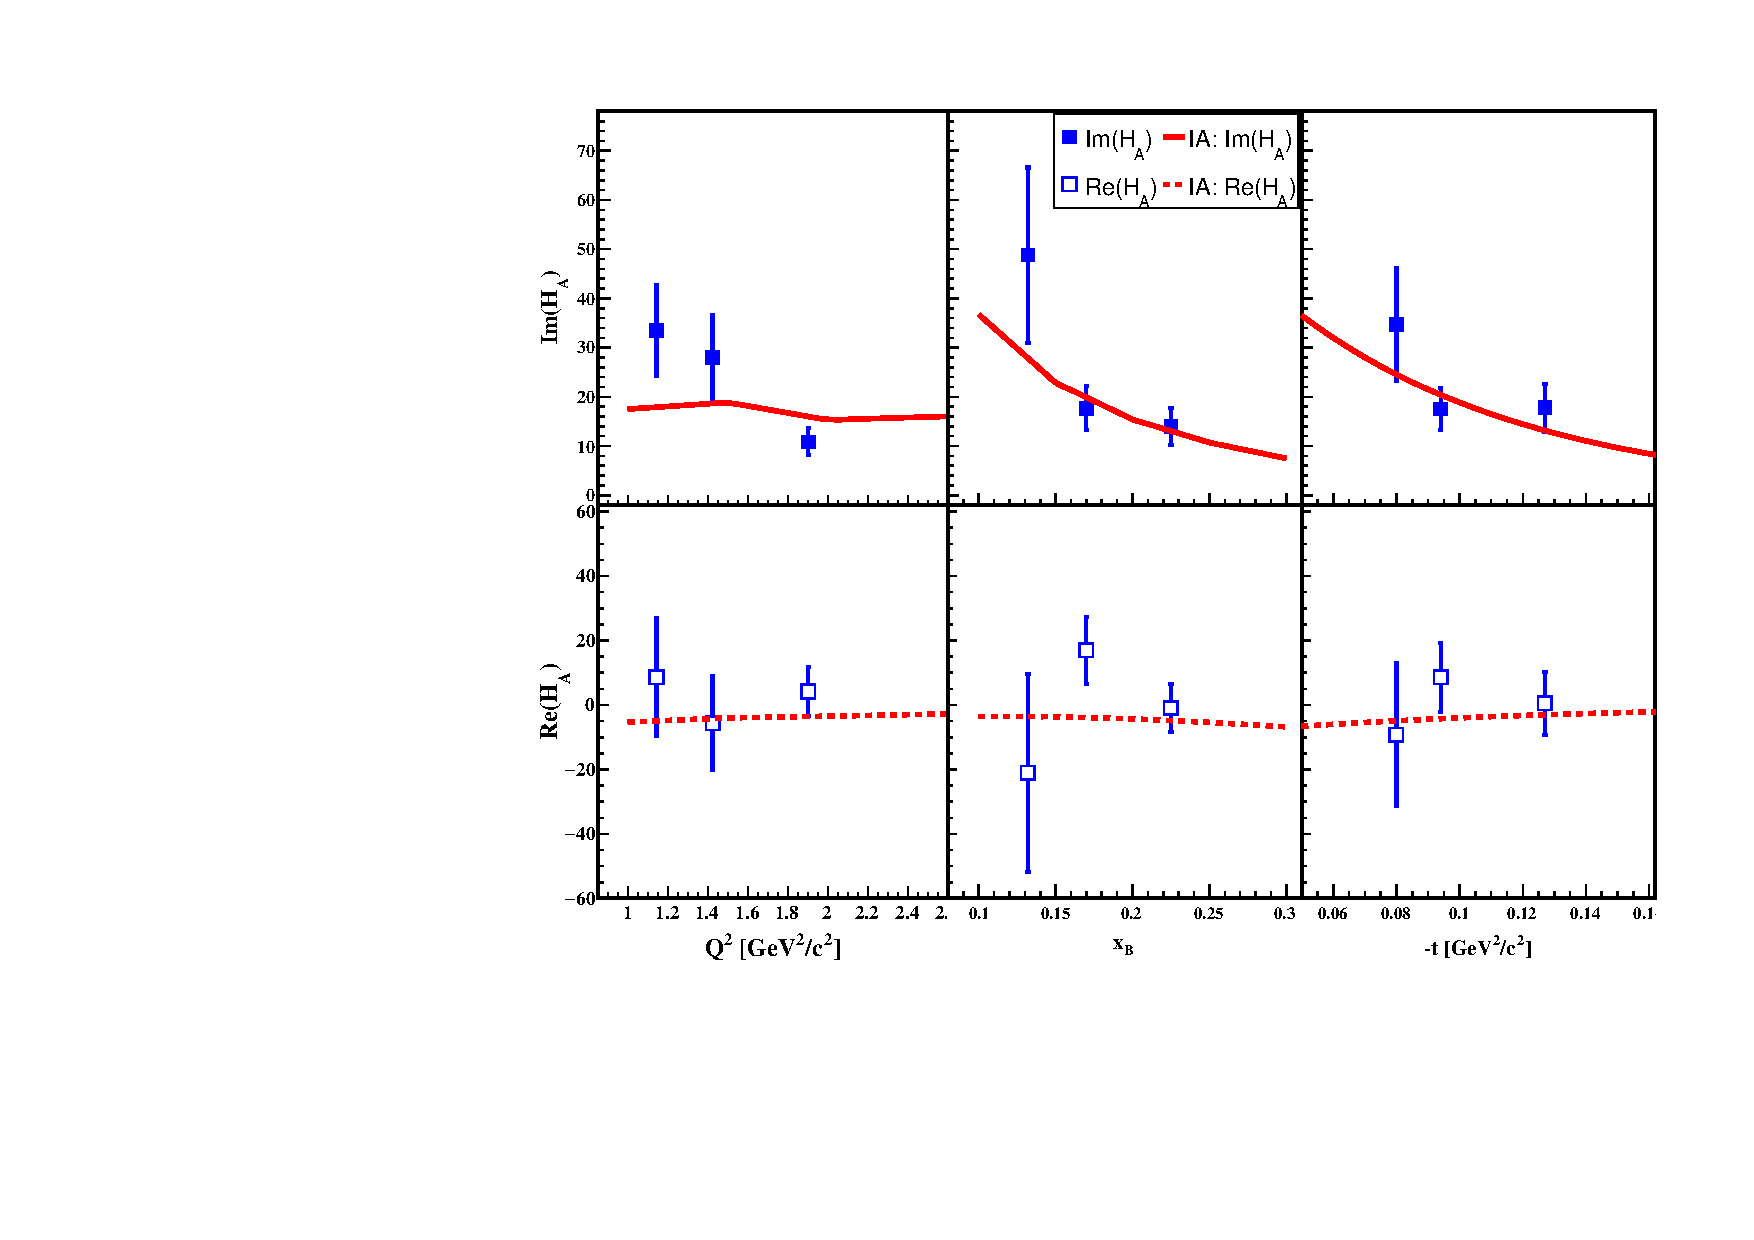
\includegraphics[width=8.9cm]{figs/updated_CFFs.pdf}
\vspace{-0.9cm}
\caption{}
\label{fig:CFF_HA}
\end{figure}



We thank the staff of the Accelerator and Physics Divisions
at Jefferson Lab for making this experiment possible.

\begin{thebibliography}{99}

\bibitem{Burkardt:2000za} 
  M.~Burkardt,
  Phys.\ Rev.\ D {\bf 62}, 071503 (2000)
  Erratum: [Phys.\ Rev.\ D {\bf 66}, 119903 (2002)]

\bibitem{Diehl:2002he} 
  M.~Diehl,
  Eur.\ Phys.\ J.\ C {\bf 25}, 223 (2002)
  Erratum: [Eur.\ Phys.\ J.\ C {\bf 31}, 277 (2003)]
 
\bibitem{Belitsky:2002ep} 
  A.~V.~Belitsky and D.~Mueller,
  Nucl.\ Phys.\ A {\bf 711}, 118 (2002)

\bibitem{Burkardt:2005hp} 
  M.~Burkardt,
  Phys.\ Rev.\ D {\bf 72}, 094020 (2005)

\bibitem{Stepanyan:2001sm}
S.~Stepanyan {\it et al.} [CLAS Collaboration],
Phys.\ Rev.\ Lett. {\bf 87}, 182002 (2001).

\bibitem{Airapetian}
A. Airapetian {\it et al.} [HERMES Collaboration],
Phys.\ Rev.\ Lett. {\bf 87}, 182001 (2001);
JHEP {\bf 1207}, 032 (2012);
JHEP {\bf 1006}, 019 (2010);
JHEP {\bf 0806}, 066 (2008);
Phys.\ Lett.\ B {\bf 704}, 15 (2011);
Phys.\ Rev.\  D {\bf 75}, 011103 (2007);
JHEP {\bf 0911}, 083 (2009);
Phys.\ Rev.\ C {\bf 81}, 035202 (2010);
JHEP {\bf 1210}, 042 (2012).

\bibitem{Chekanov:2003ya}
S. Chekanov {\it et al.} [ZEUS Collaboration],
Phys.\ Lett.\  B {\bf 573}, 46 (2003).

\bibitem{Aktas:2005ty}
A. Aktas {\it et al.} [H1 Collaboration],
Eur.\ Phys.\ J.\ C {\bf 44}, 1 (2005).

\bibitem{Chen:2006na} 
S.~Chen {\it et al.} [CLAS Collaboration],
Phys.\ Rev.\ Lett.\ {\bf 97}, 072002 (2006).

\bibitem{Munoz Camacho:2006hx} 
C. Mu\~noz Camacho {\it et al.} [Jefferson Lab Hall A Collaboration],
Phys.\ Rev.\ Lett. {\bf 97}, 262002 (2006).

\bibitem{Girod:2007aa} 
F.X. Girod {\it et al.} [CLAS Collaboration],
Phys.\ Rev.\ Lett. {\bf 100}, 162002 (2008).

\bibitem{Gavalian:2009} 
G. Gavalian {\it et al.} [CLAS Collaboration],
Phys.\ Rev.\ C {\bf 80}, 035206 (2009).

\bibitem{Seder:2015} 
E. Seder {\it et al.} [CLAS Collaboration],
Phys.\ Rev.\ Lett. {\bf 114}, 032001 (2015).

\bibitem{Pisano:2015} 
S.~Pisano {\it et al.} [CLAS Collaboration],
Phys.\ Rev.\ D {\bf 91}, 052014 (2015).

\bibitem{Jo:2015ema} 
  H.~S.~Jo {\it et al.} [CLAS Collaboration],
  Phys.\ Rev.\ Lett.\  {\bf 115}, no. 21, 212003 (2015)

\bibitem{Mazouz:2007aa} 
  M.~Mazouz {\it et al.} [Jefferson Lab Hall A Collaboration],
   Phys.\ Rev.\ Lett.\  {\bf 99}, 242501 (2007)

\bibitem{Ellinghaus:2002zw} 
  F.~Ellinghaus {\it et al.} [HERMES Collaboration],
  AIP Conf.\ Proc.\  {\bf 675}, 303 (2003)

\end{thebibliography}

\end{document}
